\documentclass[]{emulateapj}
\usepackage{amsmath}
\begin{document}
\author{Draft}


\section{Gravitational Lens model}

\subsection{interpretation}
- C06 suggest the presence of an interacting dusty galaxy in their HST observations, which BJB+08 calls it the F component. The lensed images of the ABCDE components coincide with our CO data (see mom0 on HST and channel map), evidently CO emission coming from the AGN host galaxy. 
- one of the red channels in our lens model suggests a second source component, which is consistent with the spatially offset dusty source (see mom0 on HST, which the red velocity component coincides with this F component)




\begin{figure}[tbph]
\centering
\includegraphics[width=0.50\textwidth]{../Figures/Pseudointegrated_datamodel.eps}
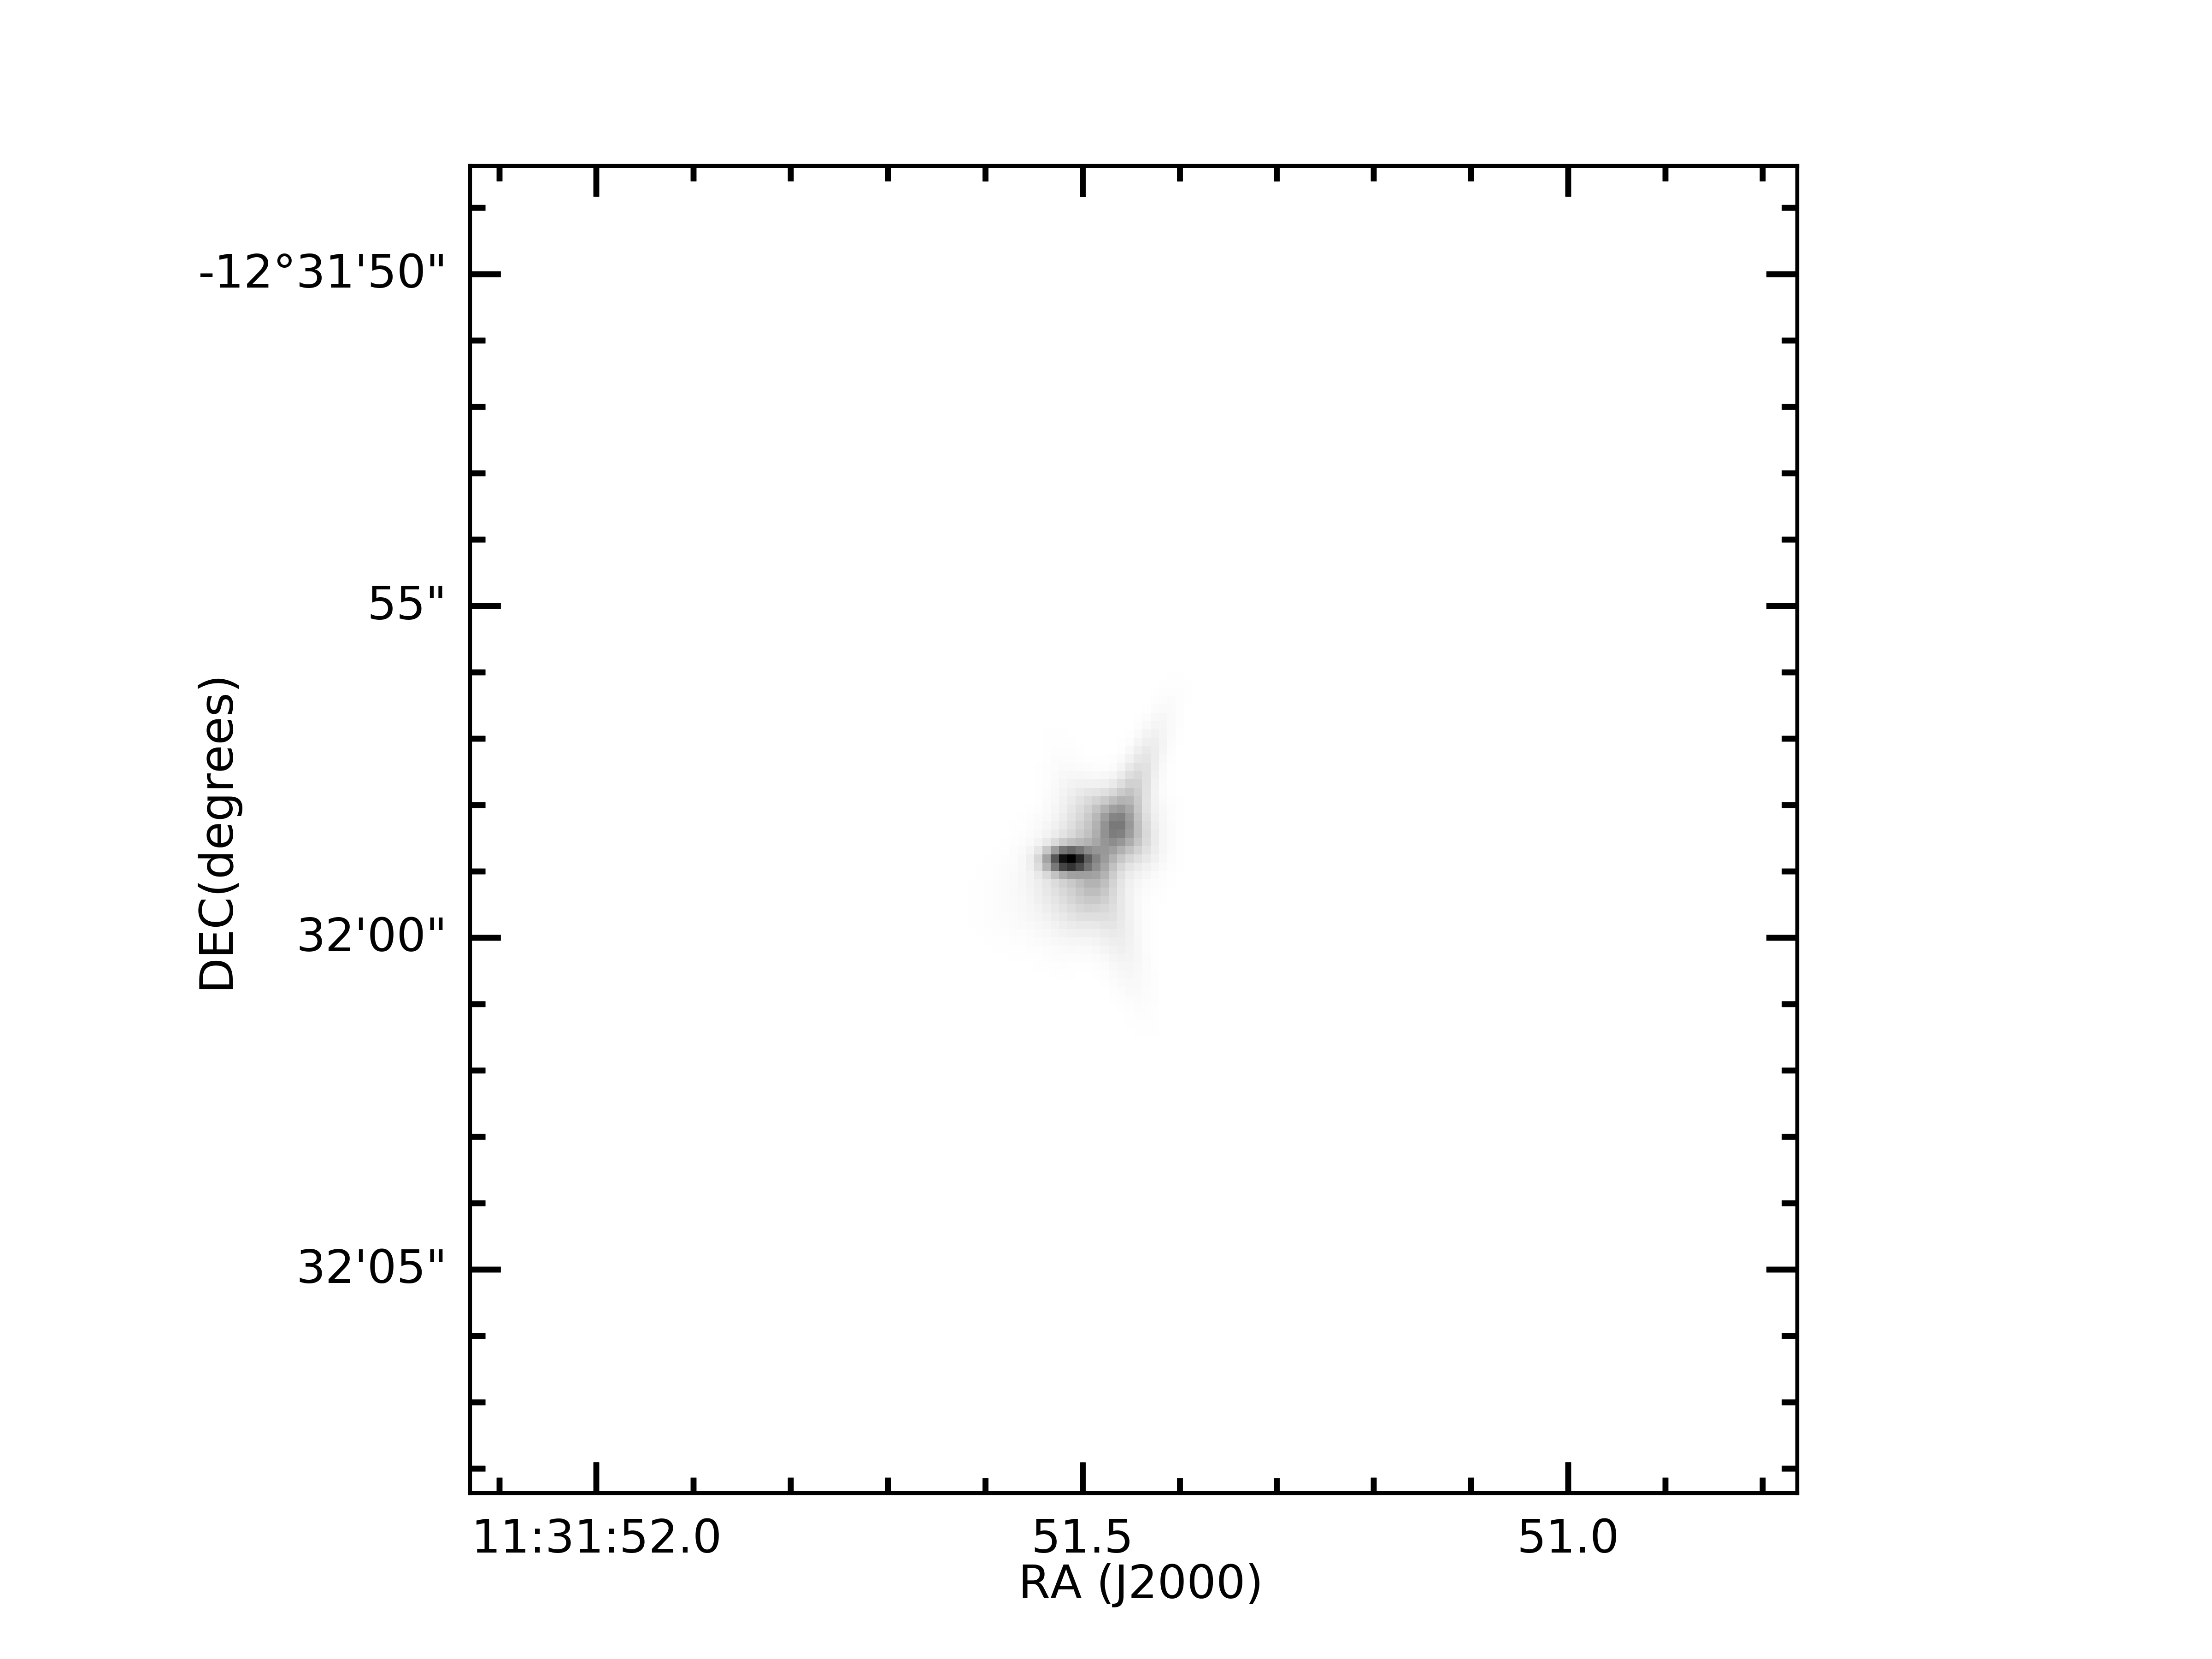
\includegraphics[width=0.50\textwidth]{../Figures/SourcesPlane.png}
\caption{
Pseudo observed 0th moment map in the lens plane. (left)
Pseudo 0th moment map in the source plane. (right)
\label{fig:}}
\end{figure}


%\begin{figure*}[tbph]
%\centering
%\caption{
%\label{fig:}}
%\end{figure*}


\begin{figure*}[tbph]
\centering
\includegraphics[width=0.80\textwidth]{../Figures/PseudoRGB_Lensed_SB_double.eps}
\caption{
velocity gradient of the lens model in the lens plane (left), source plane (right).
\label{fig:}}
\end{figure*}


%\begin{figure*}[tbph]
%\centering
%\includegraphics[width=0.8\textwidth]{}
%\includegraphics[width=0.65\textwidth]{}
%\caption{
%\label{fig:}}
%\end{figure*}

\end{document}